% !TeX spellcheck = ru_RU
\documentclass[a4paper, 14pt, unknownkeysallowed]{extreport}
\usepackage[utf8]{inputenc}
\usepackage[T2A]{fontenc}
\usepackage[english,russian]{babel}
\usepackage{cmap}
\usepackage{enumitem}

\usepackage{csvsimple}
\usepackage{hyphenat} 
\usepackage{amstext, amsmath,amsfonts,amssymb,amsthm,mathtools} 

\usepackage{setspace}
\onehalfspacing 

\usepackage{geometry}
\geometry{left=30mm}
\geometry{right=10mm}
\geometry{top=10mm}
\geometry{bottom=20mm}

\usepackage{graphicx}
\graphicspath{{img/}} 

\usepackage{threeparttable}
\usepackage{bigdelim}

\usepackage{setspace}
\onehalfspacing % Полуторный интервал

\frenchspacing
\usepackage{indentfirst} % Красная строка

\usepackage{cases}

\usepackage[unicode,pdftex]{hyperref} % Ссылки в pdf
\hypersetup{hidelinks}

\usepackage{xcolor}
\usepackage{listings}
% Для листинга кода:
\lstset{%
	language=lisp,   					% выбор языка для подсветки	
	basicstyle=\small\sffamily,			% размер и начертание шрифта для подсветки кода
	numbers=left,						% где поставить нумерацию строк (слева\справа)
	%numberstyle=,					% размер шрифта для номеров строк
	stepnumber=1,						% размер шага между двумя номерами строк
	numbersep=5pt,						% как далеко отстоят номера строк от подсвечиваемого кода
	frame=single,						% рисовать рамку вокруг кода
	tabsize=4,							% размер табуляции по умолчанию равен 4 пробелам
	captionpos=t,						% позиция заголовка вверху [t] или внизу [b]
	breaklines=true,					
	breakatwhitespace=true,				% переносить строки только если есть пробел
	escapeinside={\#*}{*)},				% если нужно добавить комментарии в коде
	backgroundcolor=\color{white},
}
\usepackage{caption}
\captionsetup{labelsep = endash}
\captionsetup[figure]{name = {}, justification = centerlast,labelformat=empty}
\captionsetup[lstlisting]{justification = justified}
\captionsetup[table]{justification = justified}


\usepackage{titlesec}
\titleformat{\chapter}{\LARGE\bfseries}{\thechapter}{20pt}{\LARGE\bfseries}
\titleformat{\section}{\Large\bfseries}{\thesection}{20pt}{\Large\bfseries}

\renewcommand\labelitemi{\ --\ }
\renewcommand\labelenumi{\theenumi)}

\newcommand{\img}[3] {
	\begin{figure}[h!]
		\includegraphics[scale = #1]{img/#2}
		\caption{#3}
		\label{img:#2}
	\end{figure}
}

\newcommand{\lst}[4]{
\lstinputlisting[language=Lisp, firstline=#1, lastline=#2, label=lst:#3,caption=#4]{sx.lsp}
}

\usepackage{siunitx,array,booktabs}


\begin{document}
% !TeX spellcheck = ru_RU
\begin{titlepage}
	
	\newgeometry{pdftex, left=2cm, right=2cm, top=2.5cm, bottom=2.5cm}
	\fontsize{12pt}{12pt}\selectfont
	\noindent \begin{minipage}{0.15\textwidth}
		
\includegraphics[width=\linewidth]{img/b_logo.jpg}
	\end{minipage}
	\noindent\begin{minipage}{0.9\textwidth}\centering
		\textbf{Министерство науки и высшего образования Российской Федерации}\\
		\textbf{Федеральное государственное бюджетное образовательное учреждение высшего образования}\\
		\textbf{«Московский государственный технический университет имени Н.~Э.~Баумана}\\
		\textbf{(национальный исследовательский университет)»}\\
		\textbf{(МГТУ им. Н.~Э.~Баумана)}
	\end{minipage}

	\noindent\rule{18cm}{3pt}
	\newline\newline
	\noindent ФАКУЛЬТЕТ $\underline{\text{«Информатика и системы управления»~~~~~~~~~~~~~~~~~~~~~~~~~~~~~~~~~~~~~~~~~~~~~~~~~~~~~~~}}$ \newline\newline
	\noindent КАФЕДРА $\underline{\text{«Программное обеспечение ЭВМ и информационные технологии»~~~~~~~~~~~~~~~~~~~~~~~}}$\newline\newline\newline\newline\newline\newline\newline
	
	
	\begin{center}
		\Large\textbf{Исследование быстродействия умножения}
		
		\Large\textbf{матриц на языке Common Lisp}
%		
		\textbf{\newline}		
	\end{center}
	
	\noindent\textbf{Студент} $\underline{\text{~~Виноградов А. О.~~~~~~~~~~~~~~~~~~~~~~~~~~~~~~~~~~~~~~~~~~~~~~~~~~~~~~~~~~~~~~~~~~~~~~~~~~~~~~~~~~~~~~}}$\newline\newline
	\noindent\textbf{Группа} $\underline{\text{~~ИУ7-66Б~~~~~~~~~~~~~~~~~~~~~~~~~~~~~~~~~~~~~~~~~~~~~~~~~~~~~~~~~~~~~~~~~~~~~~~~~~~~~~~~~~~~~~~~~~~~~~~~~~~~}}$\newline\newline
	\noindent\textbf{Преподаватель} $\underline{\text{~~Строганов Ю.В.~~~~~~~~~~~~~~~~~~~~~~~~~~~~~~~~~~~~~~~~~~~~~~~~~~~~~~~~~~~~~~~~~~~~~~~~~~~~~}}$\newline
	
	\begin{center}
		\vfill
		Москва~---~\the\year
		~г.
	\end{center}
	\restoregeometry
	
\end{titlepage}
\setcounter{page}{2}
\tableofcontents

\chapter*{Введение}
\addcontentsline{toc}{chapter}{Введение}
Цель работы: приобрести навыки использования стандартных функций Lisp.

Задачи работы:
\begin{itemize}
	\item изучить списки LISP как метод фиксации информации;
	\item изучить методы обработки списков с использованием	базовых функций Lisp.
\end{itemize}


\chapter{Теоретические вопросы}
\section{Элементы языка: определение, синтаксис, представление в памяти}
Вся информация (данные и программы) в Lisp представляется в виде символьных выражений ---  S-выражений:
\begin{equation}
	S\text{-выражение} ::= \text{<атом>} | \text{<точечная пара>}.
\end{equation}

Атомы:
\begin{itemize}
	\item символы (идентификаторы), синтаксически: набор литер (букв и цифр), начинающихся с буквы;
	\item специальные символы --- \{Т, Nil\} (используются для обозначения логических констант);
	\item самоопределимые атомы --- натуральные числа, дробные числа (например $\frac{2}{3}$), вещественные числа, строки – последовательность
	символов, заключенных в двойные апострофы (например “abc”).
\end{itemize}

Точечная пара:
\begin{align*}
	\text{<точечная пара>} &::= (\text{<атом>.<атом>}) | (\text{<атом>.<точечная пара>}) | \\
	&(\text{<точечная пара>.<атом>}) | \\
	&(\text{<точечная пара>.<точечная пара>}); \\
	\text{<список>} &::= \text{<пустой список>} | \text{<непустой список>} \\
	\text{<пустой список>} &::= ( ) | Nil \\
	\text{<непустой список>} &::= (\text{<первый элемент>.<хвост>}) \\
	\text{<первый элемент>} &::= \text{<S-выражение>} \\
	\text{<хвост>} &::= \text{<список>}
\end{align*}

%В языке Lisp при каждом выделении памяти, происходит выделение некоторого фиксированного объема, равному сумме объёмов двух адресов.
Точечная пара вида (A.B) представлена в памяти в виде двух идущих друг за другом адресов: первый указывает на A, второй --- на B.

\begin{figure}[!ht]
	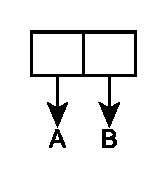
\includegraphics{pair}
	\caption{Представление в памяти точечной пары (A.B)}
	\label{fig:pair}
\end{figure}

Список представлен в памяти в виде пар ячеек, называемых списочными ячейками(пример на рисунке \ref{fig:list}). В каждой такой паре первое значение является адресом соответствующего элемента списка, второе значение --- адресом следующей пары списочной ячейки. Вторым значением списочной ячейки, соответствующей последнему элементу списка, является Nil. 

\begin{figure}[!ht]
	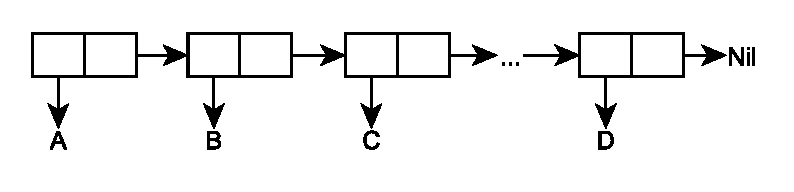
\includegraphics{list}
	\caption{Представление в памяти списка вида (A B C ... D)}
	\label{fig:list}
\end{figure}

\section{Особенности языка Lisp. Структура программы. Символ апостроф.}
Lisp --- бестиповый язык программирования. Все структуры данных, которые в нём поддерживаются, являются списками. По умолчанию, любой список расценивается как вызов функции. При чем первый элемент списка интерпретируется как сама функция, а все последующие элементы --- как ее аргументы.

Программа на языке Lisp состоит из единственного S-выражения, результат вычисления которого является результатом работы программы. Вызов функции quote отключает исчисление S-выражений. Символ апостроф --- сокращение вызова функции quote, сокращающее количество символов в программе.

\section{Базис языка Lisp. Ядро языка.}
Базисные функции Lisp:
\begin{enumerate}
	\item $quote$ --- блокировка вычислений;
	\item $eval$ --- интерпретатор;
	\item $car$ --- возвращает голову списка;
	\item $cdr$ --- возвращает хвост списка;
	\item $cons$ --- бинарная функция объединения двух параметров в точечную пару;
	\item $eq$ --- бинарная функция; будет возвращено T, если оба параметра являются одним и тем же атомом, Nil иначе;
	\item $atom$ --- унарная функция, возвращающая T, если S-выражение является атомом, Nil иначе.
	\item $cond$ --- функция произвольного числа аргументов, возвращающая результат первого выполненного условия из множества пар. Если ни одно условие не вернуло T, будет возвращено Nil.
\end{enumerate}

\chapter{Ход выполнения практического задания}
\section{Представление списков в виде списочных ячеек}

\begin{figure}[!ht]
	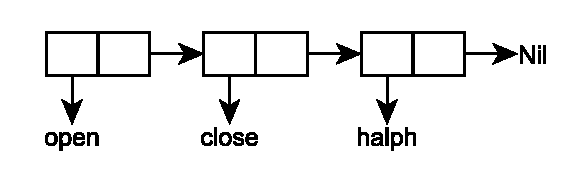
\includegraphics{task1.1}
	\caption{'(open close halph)}
\end{figure}
\begin{figure}[!ht]
	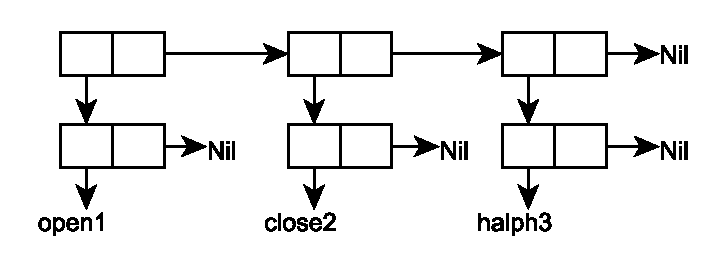
\includegraphics{task1.2}
	\caption{'((open) (close) (halph))}
\end{figure}
\begin{figure}[!ht]
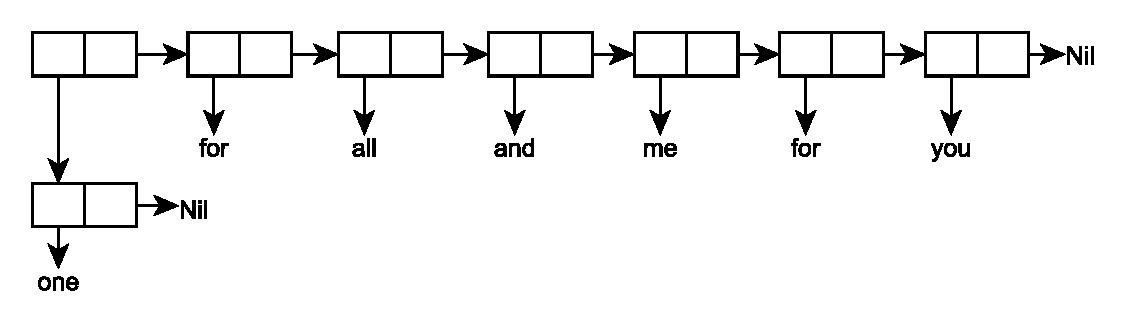
\includegraphics[width=1\linewidth]{task1.3}
\caption{'((one) for all (and (me (for you))))}
\end{figure}
\begin{figure}[!ht]
	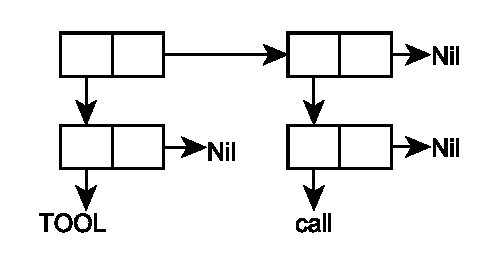
\includegraphics{task1.4}
	\caption{'((TOOL) (call))}
\end{figure}
\begin{figure}[!ht]
	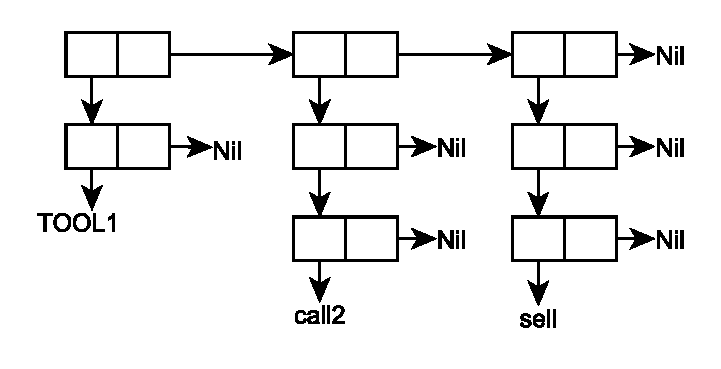
\includegraphics{task1.5}
	\caption{'((TOOL1) ((call2)) ((sell)))}
\end{figure}
\begin{figure}[!ht]
	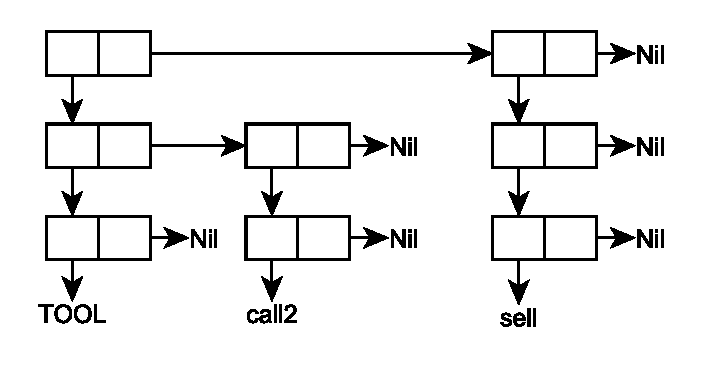
\includegraphics{task1.6}
	\caption{' (((TOOL) (call)) ((sell)))}
\end{figure}

\clearpage
\section{Используя только функции CAR и CDR, написать выражения}
Рассмотрим выражения, возвращающие 2-й, 3-й и 4-й элементы соответственно, на примере списка: '(a b c d).
\begin{enumerate}
	\item второй элемент списка --- (car (cdr '(a b c d))) = (cadr '(a b c d)) $\rightarrow$ 
	\item третий элемент списка --- (car (cdr (cdr '(a b c d)))) = (caddr '(a b c d)) $\rightarrow$
	\item четвертый элемент списка --- (car (cdr (cdr (cdr '(a b c d))))) = (cadddr '(a b c d)) $\rightarrow$
\end{enumerate}

\section{Определение результата вычисления выражений}
\begin{enumerate}
	\item (CAADR '((blue cube) (red pyramid))) --- результат: red;
	\item (CDAR '((abc) (def) (ghi))) --- результат: Nil;
	\item (CADR '((abc) (def) (ghi))) --- результат: (def);
	\item (CADDR '((abc) (def) (ghi))) --- результат: (ghi);
\end{enumerate}
\section{Результат и объяснение вычисления выражений}
\begin{enumerate}
\item (list 'Fred 'and 'Wilma) --- результат: (Fred and Wilma). list --- функция произвольного числа аргументов, формирующая список. В результате будет получен список из трех элементов. Апострофы обозначают работу с данными;
\item (list 'Fred '(and Wilma)) --- результат: (Fred (and Wilma)). Аналогичный пример; второй аргумент является списком (and Wilma).
\item (cons Nil Nil) результат: (Nil). cons --- бинарная функция объединения двух параметров в точечную пару. Так как вторым аргументом является список (Nil), точечная пара интерпретируется как список из одного элемента --- Nil.
\item (cons T Nil) --- результат: (T). Аналогично предыдущему примеру, будет получен список из одного элемента T.
\item (cons Nil T) --- результат: (Nil.T). Вторым аргументом функции cons является не список, поэтому точечная пара не приводится к списку.
\item (list Nil) --- результат: (Nil). Создан список из единственного элемента --- Nil.
\item (cons '(T) Nil) --- результат: ((T)). Аналогично рассмотренным выше случаям, второй аргумент --- список (Nil), следовательно результатом является список из одного элемента --- первого аргумента функции. Первым аргументом функции является список из одного элемента T.
\item (list '(one two) '(free temp)) --- результат: ((one two) (free temp)). Будет получен список, элементами которого являются указанные списки.
\item (cons 'Fred '(and Wilma)) --- результат: (Fred and Wilma). Точечная пара, вторым элементом которой является список, является списком.
\item (cons 'Fred '(Wilma)) --- результат: (Fred Wilma). Аналогично предыдущему номеру.
\item (list Nil Nil) --- результат: (Nil Nil). Формируем список из двух элементов.
\item (list T Nil ) --- результат: (T Nil). Формируем список из двух элементов.
\item (list Nil T) --- результат: (Nil T). Формируем список из двух элементов.
\item (cons T (list Nil)) --- результат: (T Nil). Аналогично примерам выше; точечная пара, вторым элементом которой является список (Nil).
\item (list '(T) Nil) --- результат: ((T) Nil). Формируем список из двух элементов, первый из которых является списком.
\item (cons '(one two) '(free temp)) --- результат: ((one two) free temp). Точечная пара из двух списков становится списком, элементы которого --- аргументы функции cons (списки (one two) и (free temp) в данном примере).
\end{enumerate}

\section{Лямбда-выражения и соответствующие им функции}
Написать функцию (f ar1 ar2 ar3 ar4), возвращающую список: ((ar1 ar2) (ar3 ar4)).
	\begin{itemize}
		\item (lambda (ar1 ar2 ar3 ar4) (list (list ar1 ar2) (list ar3 ar4)))
		\item (defun f (ar1 ar2 ar3 ar4) (list (list ar1 ar2) (list ar3 ar4)))
	\end{itemize}
Написать функцию (f ar1 ar2), возвращающую ((ar1) (ar2)).
	\begin{itemize}
		\item (lambda (ar1 ar2) (list (list ar1) (list ar2)))
		\item (defun f (ar1 ar2) (list (list ar1) (list ar2)))
	\end{itemize}
Написать функцию (f ar1), возвращающую (((ar1))).
	\begin{itemize}
		\item (lambda (ar1) (list (list (list ar1))))
		\item (defun f (ar1) (list (list (list ar1))))
	\end{itemize}
Представить результаты в виде списочных ячеек.

\begin{figure}[!ht]
	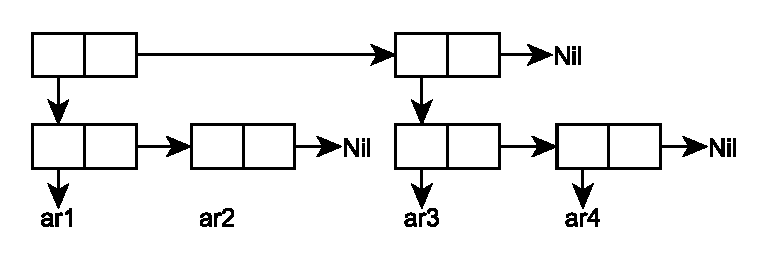
\includegraphics{task3.1}
	\caption{((ar1 ar2) (ar3 ar4))}
\end{figure}
\begin{figure}[!ht]
	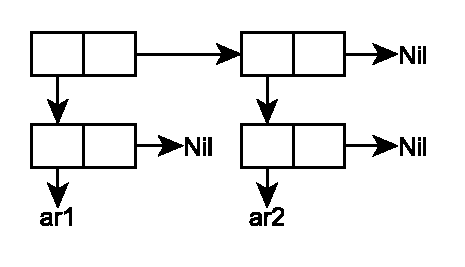
\includegraphics{task3.2}
	\caption{((ar1) (ar2))}
\end{figure}
\begin{figure}[!ht]
	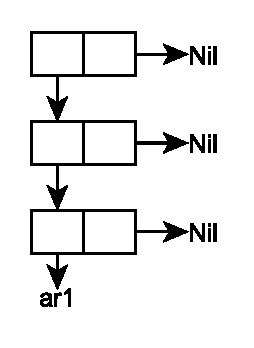
\includegraphics{task3.3}
	\caption{(((ar1)))}
\end{figure}

\chapter*{Вывод}
\addcontentsline{toc}{chapter}{Вывод}
Цель, которая была поставлена в начале лабораторной работы, была достигнута: были получены навыки использования списков и стандартных функций языка Lisp. 

Кроме того, были выполнены все поставленные задачи:
\begin{itemize}
	\item были изучены списки LISP как метод фиксации информации;
	\item были изучены методы обработки списков с использованием	базовых функций Lisp.
\end{itemize}

\end{document}